{\color{ink}\fontsize{18}{21}\selectfont\bfseries Synthetic data: increasing the probe count\par}
{\small\color{muted}Experiment results \enspace / \enspace verified 11 October 2026 \hfill 12 of 12 runs completed\par}
\vspace{4pt}
\textbf{Data.} Two $512\times512$ distance matrices, giving 262,144 coupling
variables. The source is a symmetric random metric with off-diagonal distances
uniform in $[0.5,1)$ and zero diagonal; the target is an exact permutation of it
(seed 1000, no noise or rescaling). Uniform masses are used. The planted matching
has \textbf{GW loss zero}, but the optimizer is not given that matching.

\textbf{Design.} Stochastic FraMES with 128, 1,024, 2,048 or 8,192 random-sign probes per
gradient; three development seeds (710--712), 200,000 updates each, product start
$P_0=ab^\top$, and one Ruche A100 per run. One gradient estimate is formed per
update, with $d_0=\widehat G_0$. All other settings are fixed across probe counts:
\[
 \gamma_k=(k+1)^{-3/4},\qquad
 \rho_k=0.3(k+1)^{-1/2}\ (k\geq1),\qquad
 \mu_k=\frac{10}{512}(k+1)^{-1/4}.
\]
\vspace{-5pt}
\begin{center}
\small\renewcommand{\arraystretch}{1.16}\setlength{\tabcolsep}{11pt}
\begin{tabular}{@{}rrrr@{}}
\toprule
Probes & Final feasible loss $\downarrow$ & Decrease from $P_0$ & Solver minutes\\
\midrule
128 & 0.04385652 & 0.0616\% & 12.14 \\
1,024 & 0.00004589 & 99.8954\% & 12.78 \\
2,048 & 0.00001531 & 99.9651\% & 12.62 \\
8,192 & 0.00000896 & 99.9796\% & 17.10 \\
\bottomrule
\end{tabular}
\end{center}
\vspace{-5pt}
{\small Medians across three seeds; initial feasible loss $f(P_0)=0.04388356$.
Percentage decreases are computed per seed before taking the median.}

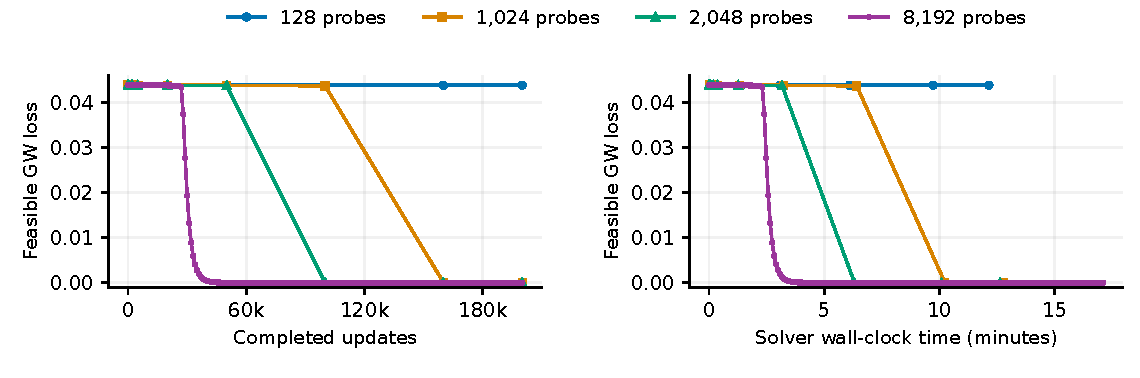
\includegraphics[width=\linewidth]{synthetic_probe_count_status_curves.pdf}
\vspace{-5pt}
{\footnotesize\color{muted}Markers are saved checkpoints; lines are visual guides. Shading shows the three-seed IQR.
The time plot places each common-iteration median loss at its median solver time; it does not interpolate to a common time grid.}

\textbf{Assessment.} All three 8,192-probe runs first show at least 99\% loss
reduction at 40,000--42,000 updates, versus a 50,000--100,000 checkpoint bracket
with 2,048. At 200,000 updates, the median final loss is 41.5\% lower, while solver
time rises from 12.6 to 17.1 minutes. The higher probe count brings the loss drop
forward; 128 probes still makes little progress.

\textbf{Scope.} The 8,192-probe runs record loss every 1,000 updates, with
additional early checkpoints. Smoothing, prefactors, seeds, start and horizon are
unchanged; GPU trajectory-parity checks passed for the added diagnostics. This
supports a probe-count effect on this clean instance, without establishing that
initial smoothing caused the delay or predicting performance on real data.

\vfill
{\footnotesize\color{muted}\textbf{Measurement.} Final-iterate loss after transport repair, evaluated in FP64;
initial and intermediate losses use FP32. This is neither a best-checkpoint loss
nor a theorem-selected output. Solver time includes initialization and updates;
it excludes preparation, repairs, loss diagnostics, logging, snapshots and final
FP64 validation. It is not end-to-end elapsed time.\\[3pt]
\textbf{Provenance.} Frozen instance \texttt{metric512\_s1000}; run sources \texttt{8d11e2a}
(128--2,048 probes) and \texttt{49911ec} (8,192). Validated report SHA256 prefixes:
\texttt{6ce0b0198875649d7} and \texttt{969f9f3b225c832a}.}
